\documentclass{article}
\usepackage[utf8]{inputenc}

\title{Project 1}
\author{Ryan Wood\\
rwood@college.harvard.edu}
\date{May 2018}

\usepackage{tikz}
\usepackage{amsmath}
\usetikzlibrary{arrows}
\usepackage{natbib}
\usepackage{graphicx}
\usepackage{amsmath}
\usepackage{enumerate}
\usepackage[margin=1.4in]{geometry}
\usepackage{fancyhdr}
\usepackage{pgfplots}
\pagestyle{fancy}
\lhead{Dr. Chen}
\chead{Project 1}
\rhead{Ryan Wood}

\begin{document}
\maketitle

\section{Separating the First Column}
We first separated the first column into four: for the personal identifiers, the number of previous arrests, the gender, and the age.\\

\begin{verbatim}
data = read.csv(fn,header = F);
info = data[c('V1')]
step1 = info %>% separate('V1', into = c('id', 'rest'), sep = "_", remove = TRUE)
step2 = step1 %>% separate('rest', into = c('goodstuff', ',jpgshit'), remove = TRUE)

step3 = step2[c('id','goodstuff')]
step3$prevarrests = NA
step3$gender = NA
step3$age = NA

#step3$prevarrests = ifelse(!is.na(as.numeric(step3$goodstuff[3])),substr(step3$goodstuff,1,1,),substr(step3$goodstuff,1,1))

for (ii in 1:length(step3[,1])) {
  if ( nchar(step3$goodstuff[ii]) == 4 ) {
    step3$prevarrests[ii] = substr(step3$goodstuff[ii],1,1)
    step3$gender[ii] = substr(step3$goodstuff[ii],2,2)
    step3$age[ii] = substr(step3$goodstuff[ii],3,4)
  }
  else if ( nchar(step3$goodstuff[ii]) == 5 ) {
    step3$prevarrests[ii] = as.numeric(substr(step3$goodstuff[ii],1,2))
    step3$gender[ii] = substr(step3$goodstuff[ii],3,3)
    step3$age[ii] = as.numeric(substr(step3$goodstuff[ii],4,5))
  }
}
step3$goodstuff = NULL
\end{verbatim}

\section{Summary Statistics for the Columns}

Now we can find some summary statistics for these columns. For the quantitative statistics, we'll return the minimum, maximum, median, 0.25 and 0.75 quantiles, and the standard deviation. For the qualitative statistic \textit{gender}, we'll just return the number of males and the number of females. At the same time, we can also plot these statistics with histograms and pie graphs.\\

\begin{verbatim}
### find summaries for previous arrests
summary(as.numeric(step3$prevarrests))
sd(as.numeric(step3$prevarrests))
hist(as.numeric(step3$prevarrests),breaks=6)

### find summaries for gender
Ms = 0
Fs = 0
for (ii in 1:length(step3$gender)) {
  if (step3$gender[ii] == 'M') {
    Ms = Ms + 1
  }
  else {
    Fs = Fs + 1
  }
}
pie(c(Ms,Fs),c('Males','Females'))

### find summaries for age
summary(as.numeric(step3$age))
sd(as.numeric(step3$age))
hist(as.numeric(step3$age),breaks=6)

### find summaries for BIFs
summary(as.numeric(unlist(data[,2:length(data[1,])])))
sd(as.numeric(unlist(data[,2:length(data[1,])])))
\end{verbatim}
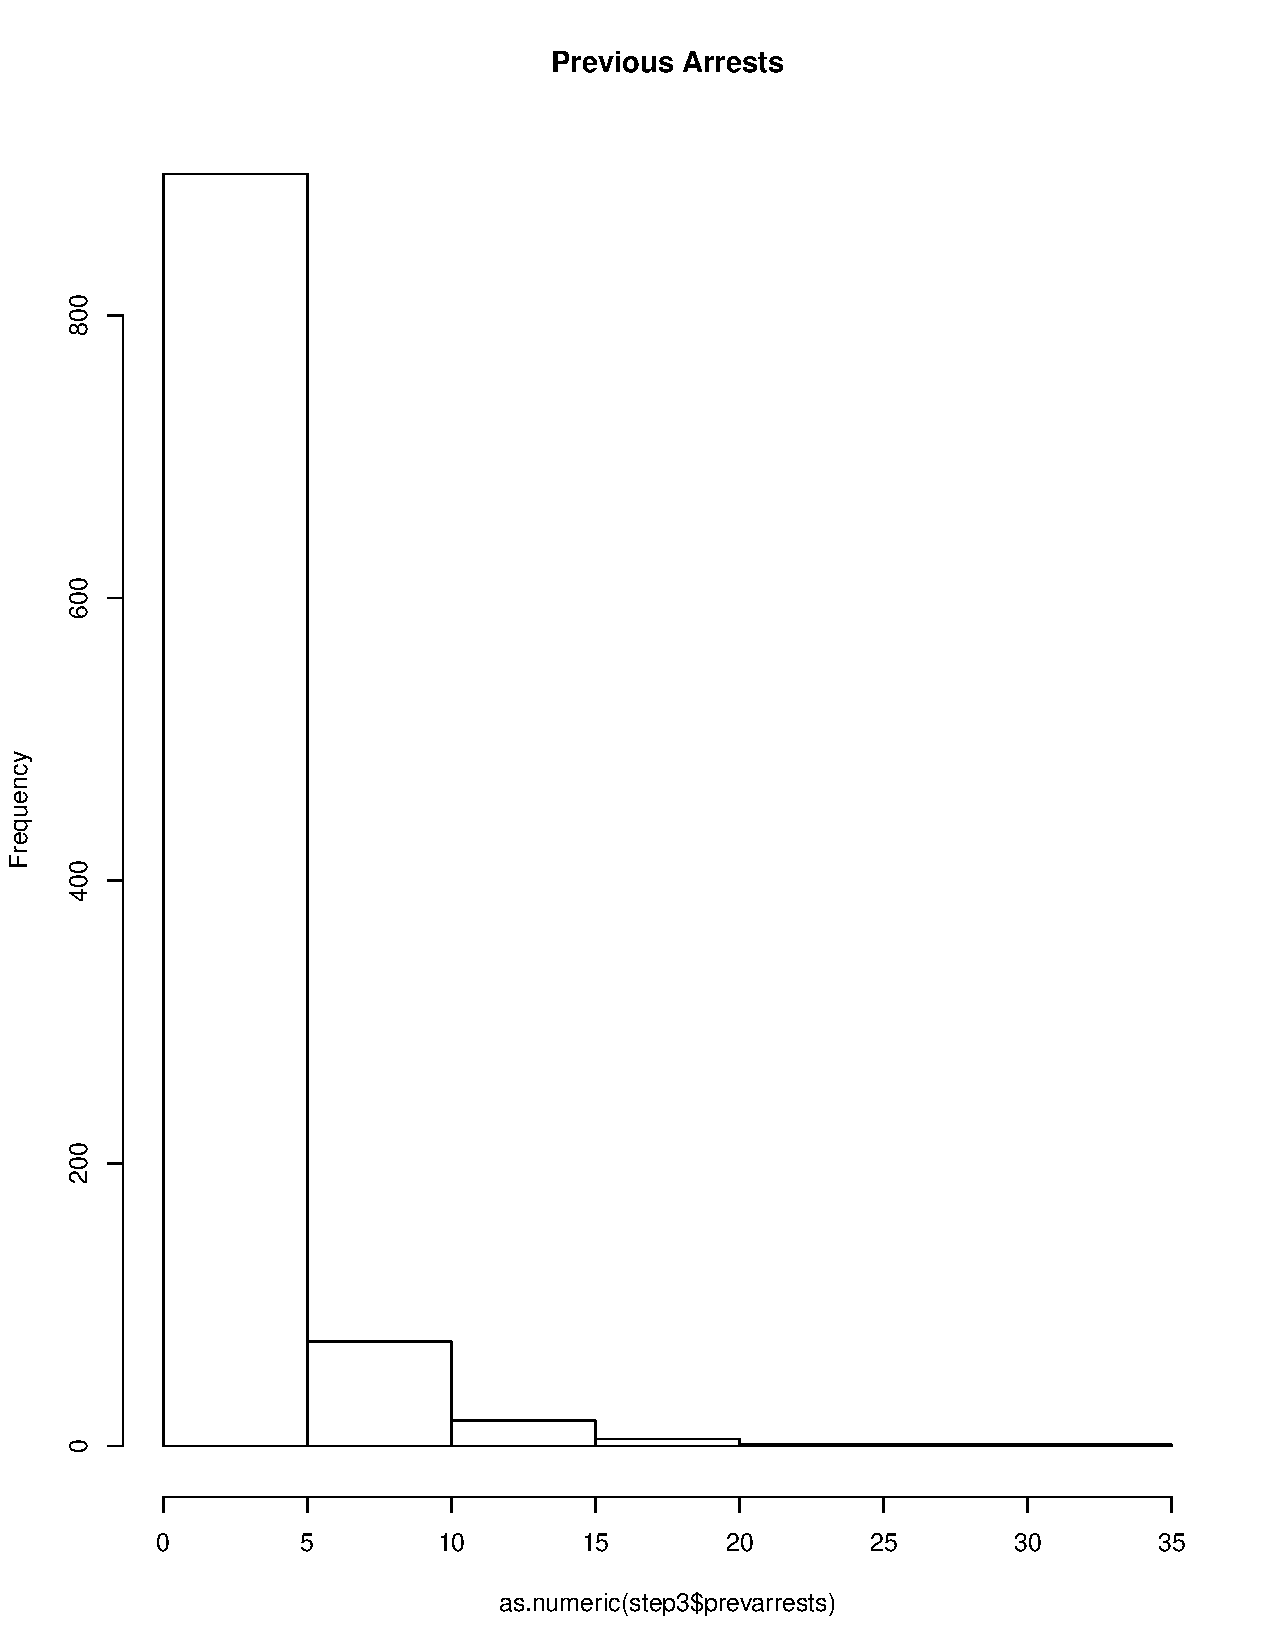
\includegraphics[width=0.7\textwidth]{PrevArrests.pdf}\\
Summary:\\
\begin{verbatim}
Min.   1st Qu.   Median  Mean   3rd Qu.    Max.    Std.
0.00    0.00     2.00    2.36    3.00     31.00  3.001234
\end{verbatim}
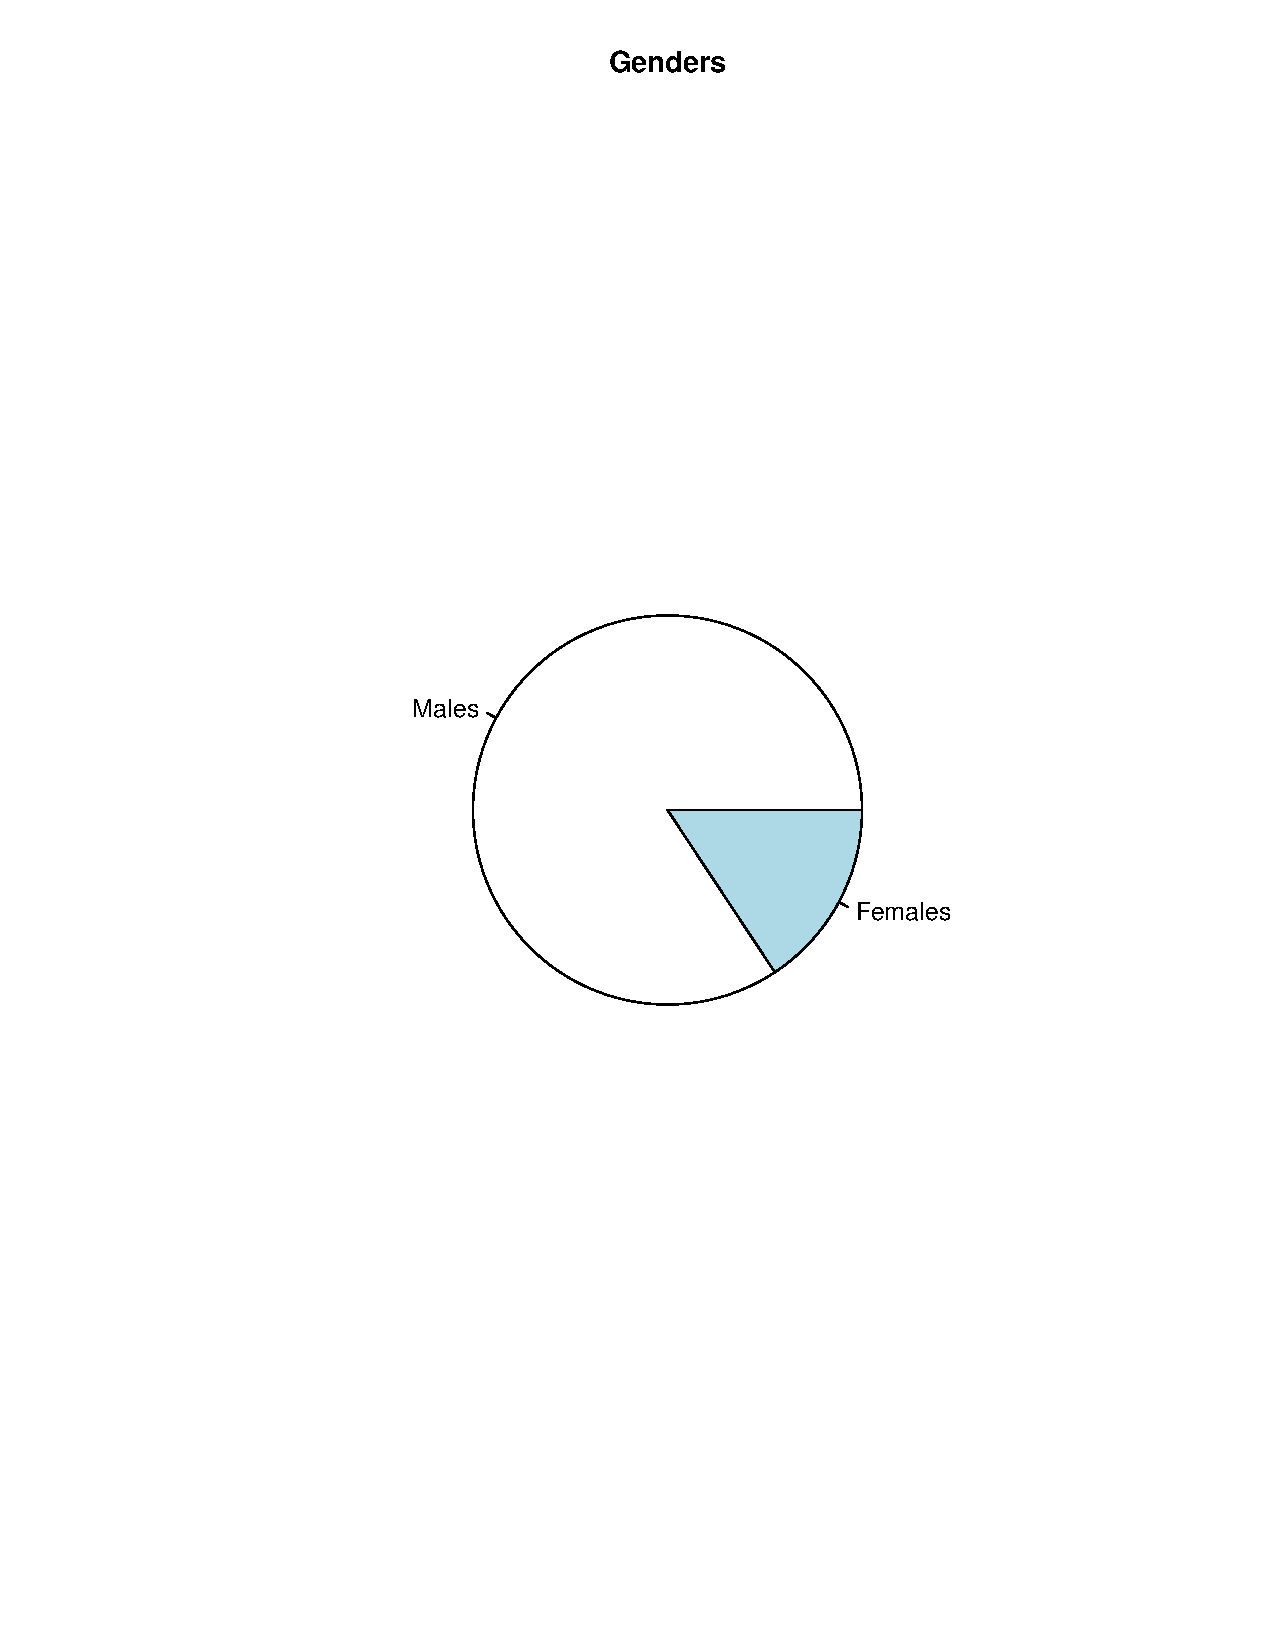
\includegraphics[width=0.7\textwidth]{Genders.pdf}\\
Summary:\\
\begin{verbatim}
Males: 843 (84.3%)
Females: 157 (15.7%)
\end{verbatim}
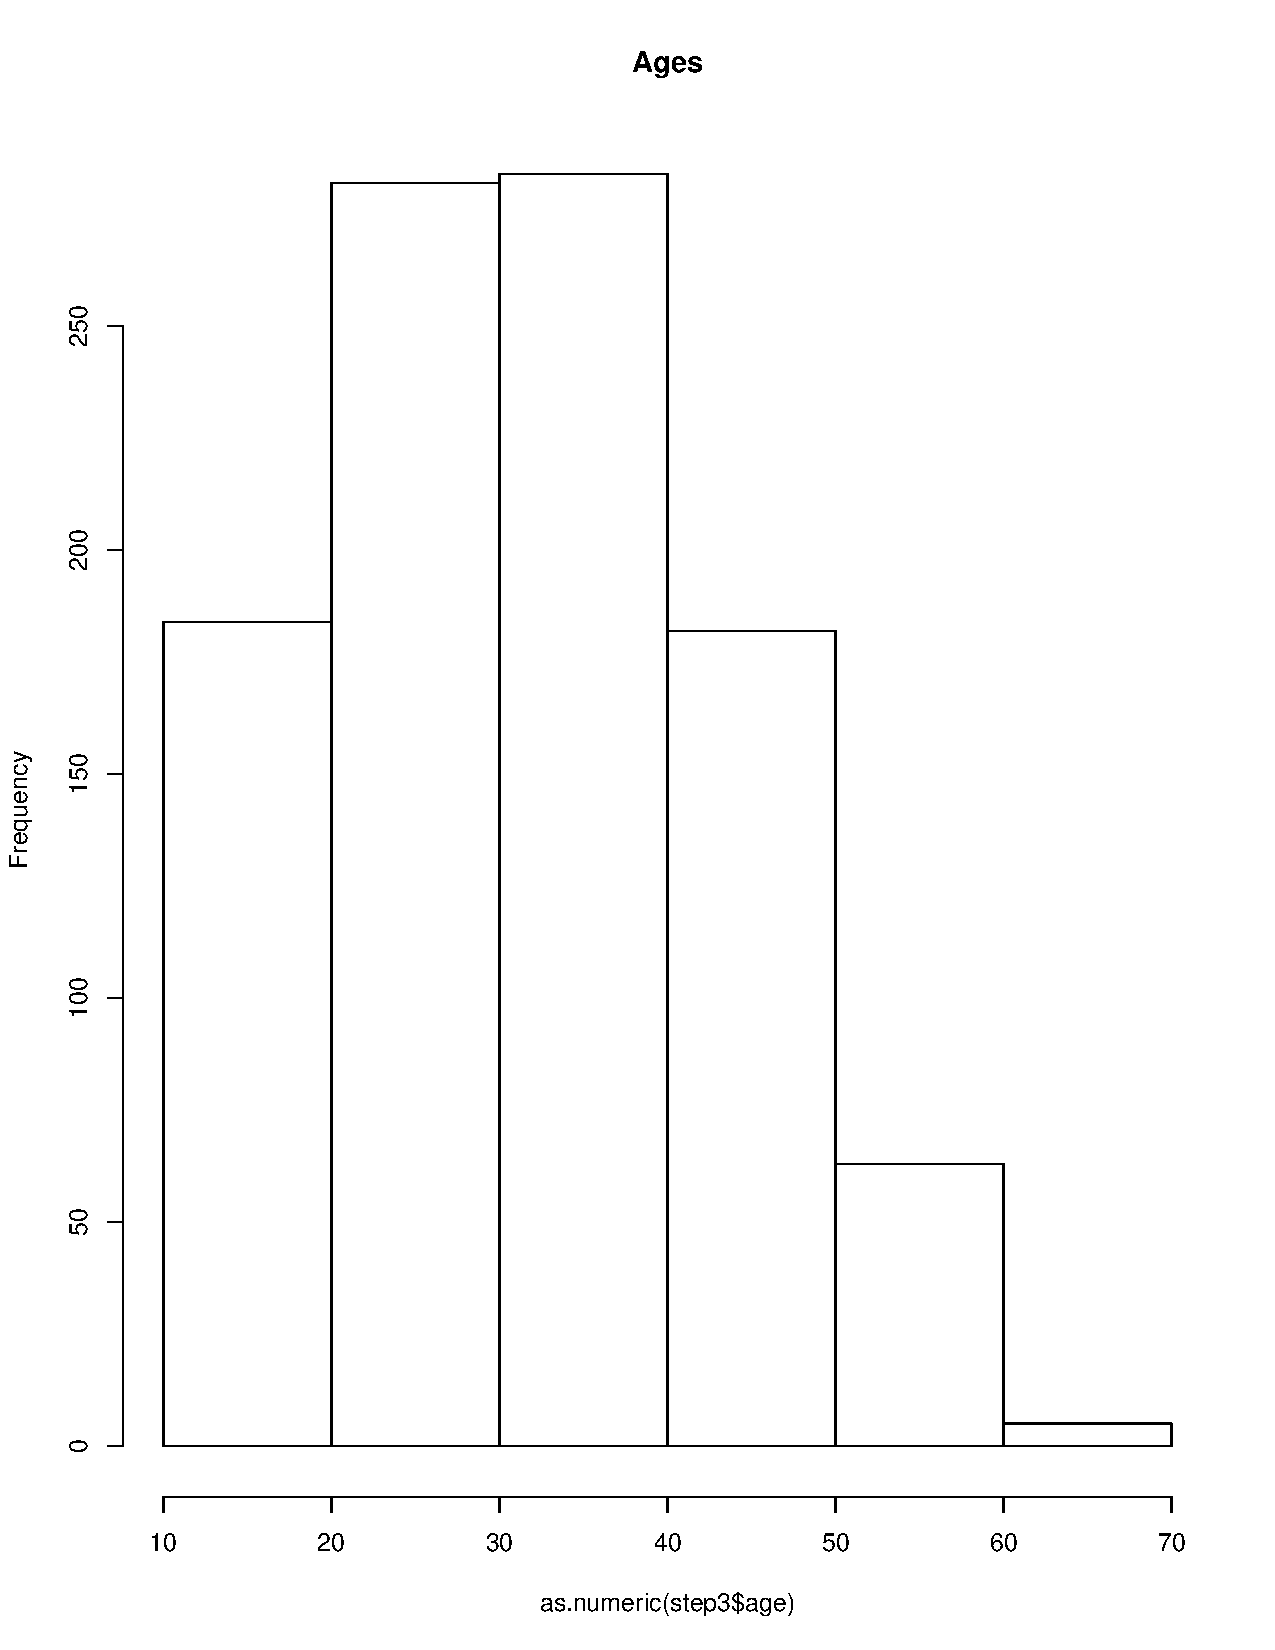
\includegraphics[width=0.7\textwidth]{Ages.pdf}\\
\begin{verbatim}
   Min. 1st Qu.  Median    Mean 3rd Qu.    Max.   Std.
  16.00   23.00   32.00   32.41   40.25   70.00 11.18172
\end{verbatim}

\section{BIFs}
The rest of the data can be considered as a whole. When taken as one set of more than 2.5 million numbers, the summary statistics are found as follows:\\
\begin{verbatim}
summary(as.numeric(unlist(data[,2:length(data[1,])])))
sd(as.numeric(unlist(data[,2:length(data[1,])])))
\end{verbatim}
\begin{verbatim}
   Min. 1st Qu.  Median    Mean 3rd Qu.    Max.   Std.
    9.0   173.0   202.0   200.1   233.0   255.0 39.06833
\end{verbatim}
We can also extract the BIF data for males and females separately as follows:\\
\begin{verbatim}
boxplot(as.numeric(unlist(data[,2:length(data[1,])]))[which(step3$gender=="M")],main="BIFs - Male")
boxplot(as.numeric(unlist(data[,2:length(data[1,])]))[which(step3$gender=="F")],main="BIFs - Female")
\end{verbatim}
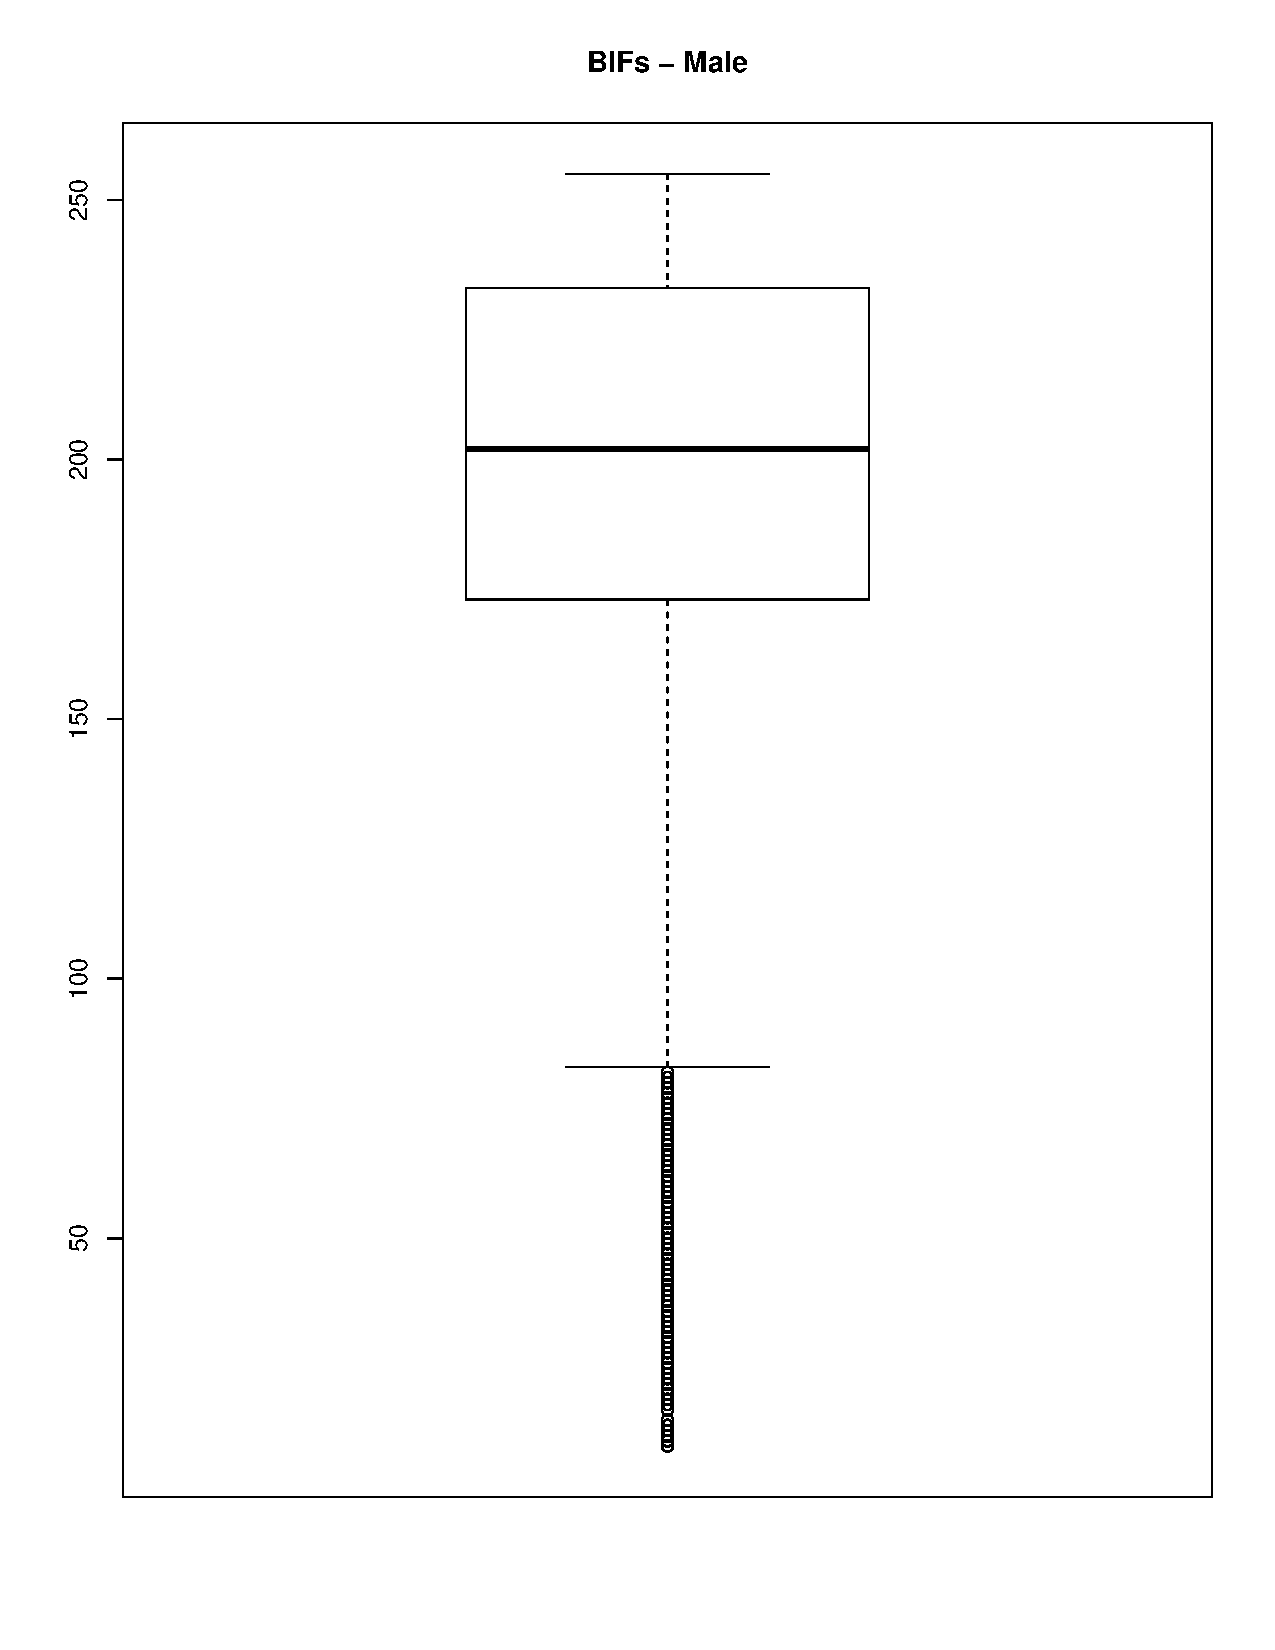
\includegraphics[width=0.5\textwidth]{BIFMale.pdf}
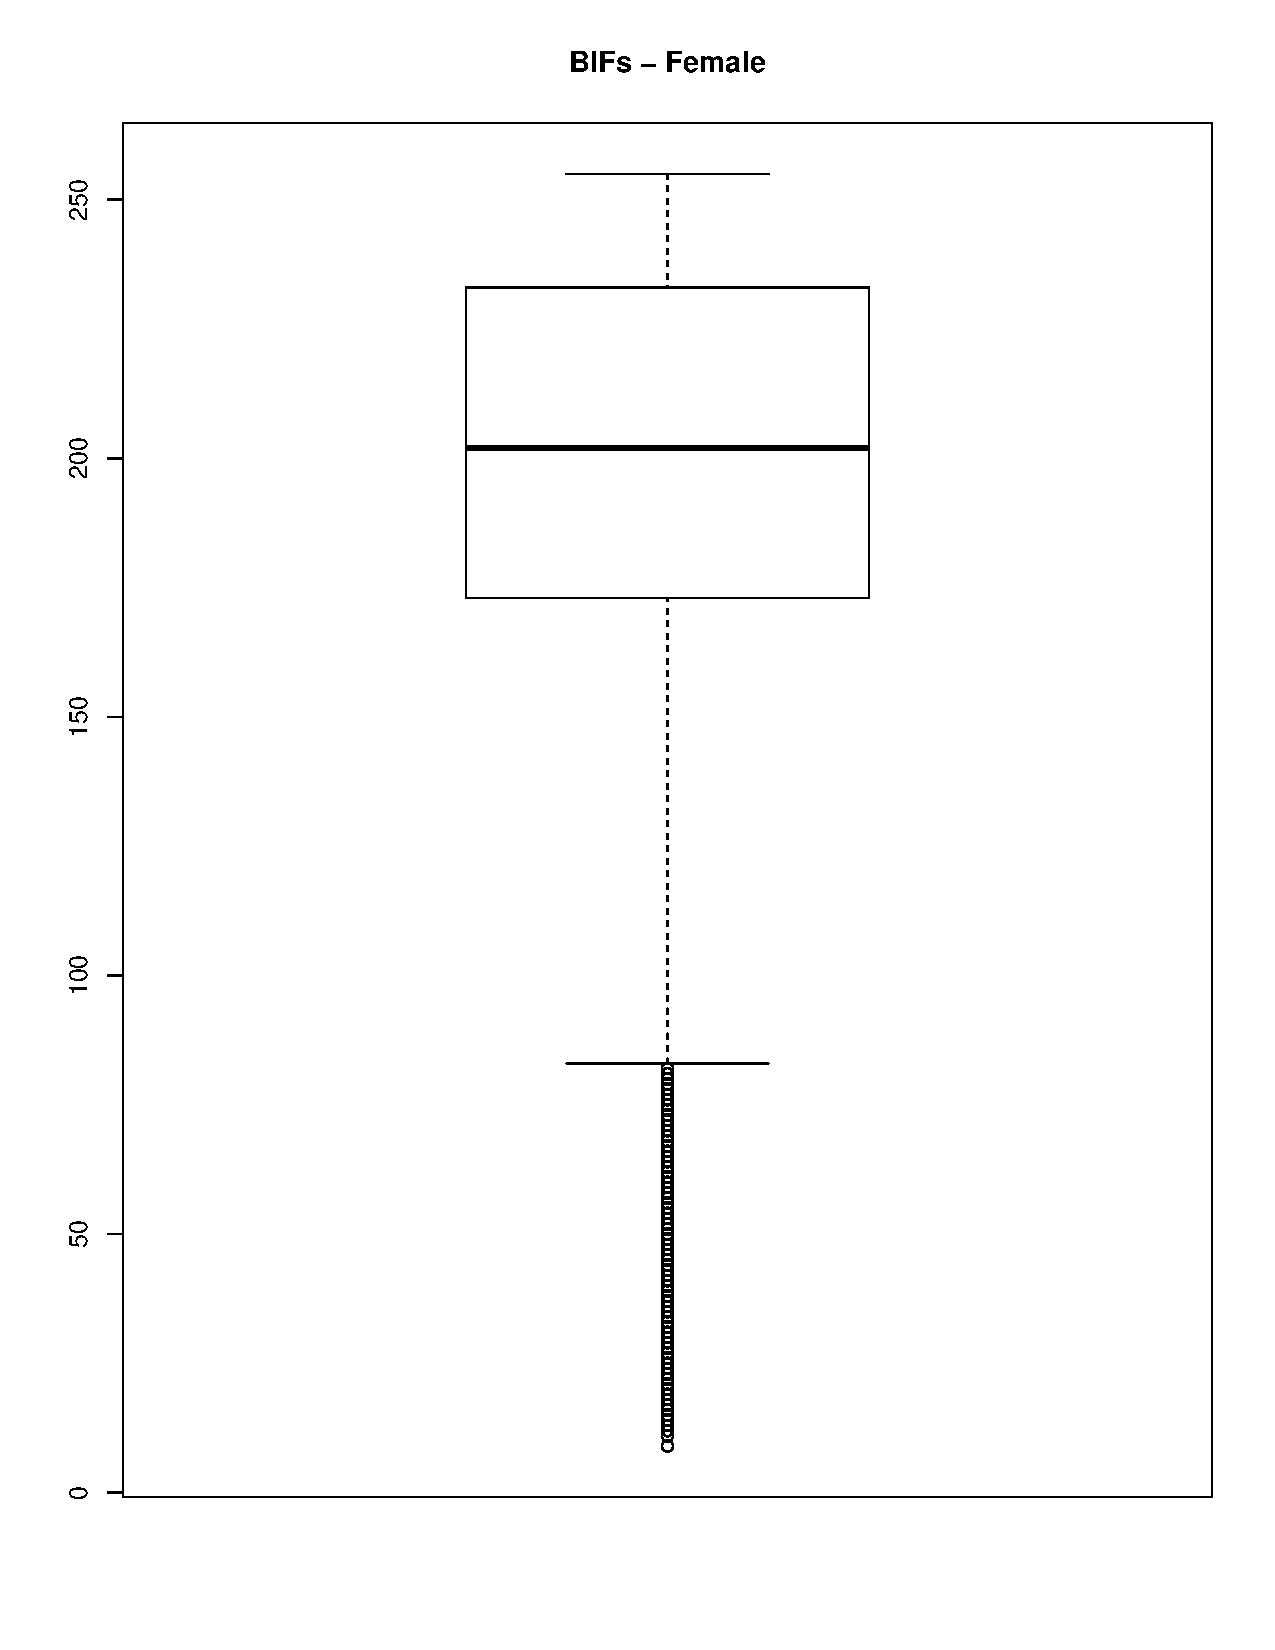
\includegraphics[width=0.5\textwidth]{BIFFemale.pdf}\\

\end{document}
